\documentclass[a4paper,class=article,border=10pt,tikz]{standalone}

%mypackages
\usepackage{pythontex}
\usepackage{pgfplots}
\usepackage{amsmath}
\usepackage{titlesec}
\usepackage{tikz}
\usetikzlibrary{shapes.geometric}
\usetikzlibrary{positioning}
\usetikzlibrary{snakes,calc,positioning,patterns,angles,quotes,decorations.pathmorphing,decorations.markings}
% \titleformat{<command>}[<shape>]{<format>}{<label>}{<sep>}{<before-code>}[<after-code>]
%\titleformat{\section}{\normalfont\Large\bfseries}{\thesection.}{10pt}{}
% \titlespacing{<command>}{<left>}{<before-sep>}{<after-sep>}
%\titlespacing{\section}{0pt}{14pt}{7pt}

%\titleformat{\subsection}{\normalfont\itshape}{\thesubsection.}{10pt}{}
%\titlespacing{\subsection}{0pt}{12pt}{6pt}
% set font encoding for PDFLaTeX, XeLaTeX, or LuaTeX
\usepackage{ifxetex,ifluatex}
\if\ifxetex T\else\ifluatex T\else F\fi\fi T%
  \usepackage{fontspec}
\else
  \usepackage[T1]{fontenc}
  \usepackage[utf8]{inputenc}
  \usepackage{lmodern}
\fi

\usepackage{hyperref}


\title{Title of Document}
\author{Name of Author}

% Enable SageTeX to run SageMath code right inside this LaTeX file.
% http://doc.sagemath.org/html/en/tutorial/sagetex.html
% \usepackage{sagetex}

% Enable PythonTeX to run Python – https://ctan.org/pkg/pythontex
% \usepackage{pythontex}

\begin{document}

 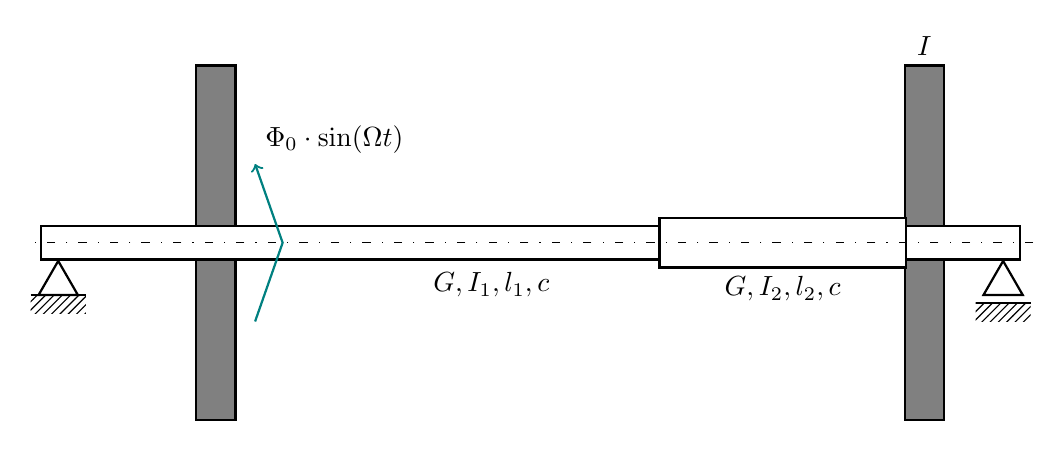
\begin{tikzpicture}

    \tikzstyle{ground}=[fill,pattern=north east lines,draw=none,minimum width=0.75cm,minimum height=0.3cm]
     \tikzstyle{close}=[draw=none,minimum width=0.75cm,minimum height=0.3cm]
    \tikzstyle{spring}=[thick,decorate,decoration={zigzag,pre length=0.3cm,post length=0.3cm,segment length=0.3cm}]
    \tikzstyle{force}=[>=stealth',ultra thick]

      \coordinate (origo) at (0,0);


\node (I_1) [fill=gray,draw,outer sep=0pt,thick,minimum width=0.5cm, xshift=-1cm,minimum height=4.5cm,label=above:{$I$}]  at (origo) {};

% \node (hole_1) [fill=white,draw,outer sep=0pt,thick,anchor=center,xshift=0cm,yshift=0cm,minimum height=0.6cm ,minimum width=0.5cm] at (I_1.center) {};



% \node (I_2) [fill=gray,draw,outer sep=0pt,thick,minimum width=0.5cm, minimum height=4.5cm,xshift=-4cm,label=above:{$I_3$}]  at (I_1) {};

% \node (hole_2) [fill=white,draw,outer sep=0pt,thick,anchor=center,xshift=0cm,yshift=0cm,minimum height=0.6cm ,minimum width=0.5cm] at (I_2.center) {};

\node (I_2) [xshift=-5cm,label=above:{$$}]  at (I_1) {};

\node (I_3) [fill=gray,draw,outer sep=0pt,thick,minimum width=0.5cm, minimum height=4.5cm, xshift=-4cm,  label=above:{}]  at (I_2) {};



% \node (hole_3) [fill=white,draw,outer sep=0pt,thick,anchor=center,xshift=0cm,yshift=0cm,minimum height=0.6cm ,minimum width=0.5cm] at (I_3.center) {};


\draw[thick,double=white,double distance=0.4cm,line cap=rect] (origo) node (start){} --++(-1cm,0) node[above=+0.3cm] (Label1){} -- ++ (-1cm,0) node (P_load){} -- ++ (-4.5cm,0) node[below=+0.25cm] (Label2){$G,I_1,l_1,c$} -- ++ (-5.5cm,0) node (shaft_end){};

\draw[thick,double=white,double distance=0.6cm,line cap=rect] ([xshift=-0.3cm]I_1.west) --++(-2.5cm,0) node[midway,below=0.3cm] {$G,I_2,l_2,c$};


\draw [thin, loosely dashdotted] ([xshift=0.25cm]start.east) --([xshift=-0.25cm]shaft_end.west);

% \draw[thick] (shaft_end.north) -- (shaft_end.south);
% \draw[thick] (start.north) -- (start.south);

\draw[thick, teal,->] (I_3)++(0.5cm,-1cm)  --++(0.35cm,1cm) --++ (-0.35cm,1cm) node[above right, black] {${\Phi_{0}} \cdot{\sin({\Omega}{t})}$};

% \draw [spring]  (I_1.north west) ++ (0cm,-0.5cm) -- ([yshift=-0.5cm]I_2.north east) node (k)[above,midway] {$k$};

% \draw [spring]  (I_1.south west) ++ (0cm,+0.5cm) -- ([yshift=+0.5cm]I_2.south east) node (k)[above,midway] {$k$};


% \draw [spring]  (I_2.north west) ++ (0cm,-0.5cm) -- ([yshift=-0.5cm]I_3.north east) node (k)[above,midway] {$\kappa$};

% \draw [spring]  (I_2.south west) ++ (0cm,+0.5cm) -- ([yshift=+0.5cm]I_3.south east) node (k)[above,midway] {$\kappa$};


\draw [thick] ([yshift=-0.1cm]shaft_end.south) --++ (-60:0.5) --++(-0.5,0) node (support_end) {} --++ (60:0.5)  ;
\node (fixed_support) [ground,outer sep=0pt,thick,anchor=north west,xshift=-0.1cm,yshift=0cm,minimum height=0.1cm ,minimum width=0.7cm]  at (support_end) {};

\draw [thick] (fixed_support.north west) -- (fixed_support.north east);

\draw [thick] ([yshift=-0.1cm]start.south) --++ (-60:0.5) --++(-0.5,0)  node (support_start) {}  --++ (60:0.5);

\node (floating_support) [ground,outer sep=0pt,thick,anchor=north west,xshift=-0.1cm,yshift=-0.1cm,minimum height=0.05cm ,minimum width=0.7cm]  at (support_start) {};

\draw [thick] (floating_support.north west) -- (floating_support.north east);

%     \draw [color=teal,force,<-]  (origo) -- ++(+1.5cm,0) node [above](Rxz){$F_{1x}$};
     % \draw [color=teal,force,<-]  (origo) -- ++(0cm,1.5cm) node [left](Ryz){$F_{1y}$};
%      \draw [color=teal,force,->]  (origo) -- ([shift=(140:0.75cm)]origo) arc (140:30:0.75cm) node[above=0.25cm](M_fix) {$M_1$};
%
%
%      \draw [color=teal,force,<-]  (R_wheel.center) -- ++(-1.5cm,0) node [above](Rxz){$F_{2x}$};
%      \draw [color=teal,force,->]  (R_wheel) -- ++(0cm,1.5cm) node [left](Ryz){$F_{2y}$};
%      \draw [color=teal,force,->]  (R_wheel.center) -- ([shift=(140:0.75cm)]R_wheel.center) arc (140:30:0.75cm) node[above=0.25cm](M_fix) {$M_2$};

     % \draw[thin,->]  (R_wheel) -- ++(0cm,-0.75cm)  --++(+1cm,0cm) node[midway, above](x_1){$x_1$};
%     \draw[thin,->]  (P_load) -- ++(0cm,-0.75cm)  --++(+1cm,0cm) node[midway, above](x_2){$x_2$};
\end{tikzpicture}
\end{document}
% \draw[<->,line width=1.5pt] (-0.5,0)--(0.5,0) node[midway,above]{$x_{e}(t)$};
